
\chapter{Implementierungsplan und Implementierungsdurchführung}
In diesem Abschnitt wird die Implementierung des Prototypen genau geplant. Für die Planung haben sich die Gruppenmitglieder der STH-App in gemeinsamen Meetings abgestimmt. Im folgenden werden die Schritte genauer erläutert.

\section{Teilprojekte und Arbeitspakete}
In diesem Kapitel liegt der Fokus auf den Arbeitspaketen, die für die Entwicklung der STH-App von entscheidender Bedeutung sind. Es wird zunächst erläutert, welche Aufgabenstellung jedes Arbeitspaket initialisiert, wobei sowohl die Verantwortlichen des Arbeitspakets als auch die damit verbundenen Ressourcen betrachtet werden.
\\
\\
\\
\textbf{Definition der Arbeitspakete:} \\

\textbf{Arbeitspaket 1 vom 08.03.2024 bis 11.03.2024}
\begin{itemize}[itemsep=0pt]
    \item{Bezeichnung: Initial Setup Flutter} 
    \item{Verantwortliche/r: Das Team} 
    \item{Ressourcen: VS Code, Flutter SDK, Android Emulator und iOS Simulator} 
    \item{Aufgabenstellung: Einrichtung der Entwicklungsumgebung für Flutter}
\end{itemize} 

\textbf{Arbeitspaket 2 vom 08.03.2024 bis 11.03.2024}
\begin{itemize}[itemsep=0pt]
    \item{Bezeichnung: Initial Setup LaTeX} 
	\item{Verantwortliche/r: Das Team} 
	\item{Ressourcen: VS Code incl\. LaTeX-Plugins, Container-Plattform (Docker)} 
	\item{Aufgabenstellung: Einrichtung der Entwicklungsumgebung für LaTeX}
\end{itemize}

\textbf{Arbeitspaket 3 vom 08.03.2024 bis 11.03.2024}
\begin{itemize}[itemsep=0pt]
    \item{Bezeichnung: Initial Setup GitHub} 
	\item{Verantwortliche/r: Das Team} 
	\item{Ressourcen: Git-Client, GitHub-Konto} 
	\item{Aufgabenstellung: Erstellung des Repositories auf GitHub}
\end{itemize}

\newpage
\textbf{Arbeitspaket 4 vom 13.03.2024 bis 14.03.2024}
\begin{itemize}[itemsep=0pt]
    \item{Bezeichnung: Project Roadmap} 
	\item{Verantwortliche/r: Das Team} 
	\item{Ressourcen: Brainstorming} 
	\item{Aufgabenstellung: Definition der App Funktionalitäten}
\end{itemize} 

\textbf{Arbeitspaket 5 vom 14.03.2024 bis 15.03.2024}
\begin{itemize}[itemsep=0pt]
    \item{Bezeichnung: Project Structure} 
	\item{Verantwortliche/r: Herr Jonas Waigel} 
	\item{Ressourcen: VS Code, Flutter Framework} 
    \item{Aufgabenstellung: Erstellung der ersten Projektstruktur in Visual Studio Code und Flutter}
\end{itemize}

\textbf{Arbeitspaket 6 vom 15.03.2024 bis 22.03.2024}
\begin{itemize}[itemsep=0pt]
    \item{Bezeichnung: Home-Screen} 
	\item{Verantwortliche/r: Herr Jonas Waigel} 
	\item{Ressourcen: VS Code, Flutter Framework} 
    \item{Aufgabenstellung: Implementierung des Home-Screens inklusive Menüleiste (Bottom Navigationbar) am unteren Bildschirmrand und App Bar am oberen Bildschirmrand}
\end{itemize}

\textbf{Arbeitspaket 7 vom 18.03.2024 bis 01.04.2024}
\begin{itemize}[itemsep=0pt]
    \item{Bezeichnung: Chat-Screen} 
	\item{Verantwortliche/r: Herr Hasan Deveci} 
	\item{Ressourcen: VS Code, Flutter Framework} 
    \item{Aufgabenstellung: Implementierung des Chat-Screens}
\end{itemize} 

\textbf{Arbeitspaket 8 vom 21.03.2024 bis 04.04.2024}
\begin{itemize}[itemsep=0pt]
    \item{Bezeichnung: Account Profile} 
	\item{Verantwortliche/r: Herr Fitim Makolli} 
	\item{Ressourcen: VS Code, Flutter Framework} 
    \item{Aufgabenstellung: Implementierung des Account-Profile-Screens inklusive Avatar und personenbezogene Daten}
\end{itemize}

\newpage
\textbf{Arbeitspaket 9 vom 22.03.2024 bis 05.04.2024}
\begin{itemize}[itemsep=0pt]
    \item{Bezeichnung: Search-Screen} 
	\item{Verantwortliche/r: Herr Vatsegkan Zournatsidis} 
	\item{Ressourcen: VS Code, Flutter Framework} 
    \item{Aufgabenstellung: Initiale Implementierung des Search-Screens}
\end{itemize}

\textbf{Arbeitspaket 10 vom 22.03.2024 bis 01.04.2024}
\begin{itemize}[itemsep=0pt]
    \item{Bezeichnung: Global-Menu-Bar} 
	\item{Verantwortliche/r: Herr Jonas Waigel} 
	\item{Ressourcen: VS Code, Flutter Framework} 
    \item{Aufgabenstellung: Implementierung einer globalen Menüleiste am unteren Bildschirmrand für alle Pages}
\end{itemize} 

\textbf{Arbeitspaket 11 vom 25.03.2024 bis 08.04.2024}
\begin{itemize}[itemsep=0pt]
    \item{Bezeichnung: Initial Setup Backend} 
	\item{Verantwortliche/r: Herr Jonas Waigel} 
	\item{Ressourcen: VS Code, Flutter Framework, Backend-Plattform (Firebase)}
    \item{Aufgabenstellung: Backend-Initialisierung (Firebase)}
\end{itemize}

\textbf{Arbeitspaket 12 vom 25.03.2024 bis 01.04.2024}
\begin{itemize}[itemsep=0pt]
    \item{Bezeichnung: Profile-Edit-Button} 
	\item{Verantwortliche/r: Herr Fitim Makolli} 
	\item{Ressourcen: VS Code, Flutter Framework} 
    \item{Aufgabenstellung: Implementierung eines Bearbeitungsbuttons für den Account-Profile-Screen}
\end{itemize}

\textbf{Arbeitspaket 13 vom 25.03.2024 bis 01.04.2024}
\begin{itemize}[itemsep=0pt]
    \item{Bezeichnung: Logo Design} 
	\item{Verantwortliche/r: Herr Vatsegkan Zournatsidis} 
	\item{Ressourcen: ChatGPT 4.0}
    \item{Aufgabenstellung: Gestaltung eines Logos für die STH-APP}
\end{itemize} 

\textbf{Arbeitspaket 14 vom 25.03.2024 bis 04.04.2024}
\begin{itemize}[itemsep=0pt]
    \item{Bezeichnung: Loading-Screen} 
	\item{Verantwortliche/r: Herr Vatsegkan Zournatsidis} 
	\item{Ressourcen: VS Code, Flutter Framework} 
    \item{Aufgabenstellung: Implementierung einer Ladebildschirm-Funktion beim Start der STH-App}
\end{itemize}

\textbf{Arbeitspaket 15 vom 27.03.2024 bis 05.04.2024}
\begin{itemize}[itemsep=0pt]
    \item{Bezeichnung: GetStream-Chat} 
	\item{Verantwortliche/r: Herr Hasan Deveci} 
	\item{Ressourcen: VS Code, Flutter Framework} 
    \item{Aufgabenstellung: Implementierung von GetStream-Chat}
\end{itemize}

\textbf{Arbeitspaket 16 vom 27.03.2024 bis 28.03.2024}
\begin{itemize}[itemsep=0pt]
    \item{Bezeichnung: Chat-App-Bar}
	\item{Verantwortliche/r: Herr Jonas Waigel} 
	\item{Ressourcen: VS Code, Flutter Framework} 
    \item{Aufgabenstellung: Anpassung der App-Leiste auf dem Chat-Screen}
\end{itemize} 

\textbf{Arbeitspaket 17 vom 29.03.2024 bis 04.04.2024}
\begin{itemize}[itemsep=0pt]
    \item{Bezeichnung: Logo Loading-Screen} 
	\item{Verantwortliche/r: Herr Vatsegkan Zournatsidis} 
	\item{Ressourcen: VS Code, Flutter Framework} 
    \item{Aufgabenstellung: Implementierung eines Loading-Screen mit einem Logo}
\end{itemize}

\textbf{Arbeitspaket 18 vom 01.04.2024 bis 08.04.2024}
\begin{itemize}[itemsep=0pt]
    \item{Bezeichnung: Backend Config} 
	\item{Verantwortliche/r: Herr Jonas Waigel} 
	\item{Ressourcen: VS Code, Flutter Framework, Backend-Plattform (Firebase)}
    \item{Aufgabenstellung: Implementierung der Backend-Konfiguration (Firebase), Authentifizierung und deren Methoden} 
\end{itemize}

\textbf{Arbeitspaket 19 vom 01.04.2024 bis 08.04.2024}
\begin{itemize}[itemsep=0pt]
    \item{Bezeichnung: Custom Page Routing} 
	\item{Verantwortliche/r: Herr Jonas Waigel} 
	\item{Ressourcen: VS Code, Flutter Framework} 
    \item{Aufgabenstellung: Implementierung einer benutzerdefinierten Seitenroute beim Wechsel von Pages}
\end{itemize} 

\textbf{Arbeitspaket 20 vom 02.04.2024 bis 08.04.2024}
\begin{itemize}[itemsep=0pt]
    \item{Bezeichnung: Chat UI Adjustments} 
	\item{Verantwortliche/r: Herr Hasan Deveci} 
	\item{Ressourcen: VS Code, Flutter Framework} 
    \item{Aufgabenstellung: Anpassung des Chat-Screens und der benutzerdefinierte App-Leiste}
\end{itemize}

\textbf{Arbeitspaket 21 vom 02.04.2024 bis 08.04.2024}
\begin{itemize}[itemsep=0pt]
    \item{Bezeichnung: Channel Adjustment} 
	\item{Verantwortliche/r: Herr Hasan Deveci} 
	\item{Ressourcen: VS Code, Flutter Framework} 
    \item{Aufgabenstellung: Anpassung des Chanels im Chat-Screen}
\end{itemize}

\textbf{Arbeitspaket 22 vom 02.04.2024 bis 03.04.2024}
\begin{itemize}[itemsep=0pt]
    \item{Bezeichnung: Latex Docs Update} 
	\item{Verantwortliche/r: Herr Jonas Waigel} 
	\item{Ressourcen: VS Code} 
    \item{Aufgabenstellung: Aufgabenstellung: Dokumentationsstruktur in LaTeX aktualisieren}
\end{itemize} 

\textbf{Arbeitspaket 23 vom 03.04.2024 bis 10.04.2024}
\begin{itemize}[itemsep=0pt]
    \item{Bezeichnung: Local Storage Setup} 
	\item{Verantwortliche/r: Herr Fitim Makolli} 
	\item{Ressourcen: VS Code, Flutter Framework} 
    \item{Aufgabenstellung: Implementierung eines lokalen Speichers für den Account-Profile-Screen}
\end{itemize}

\textbf{Arbeitspaket 24 vom 03.04.2024 bis 10.04.2024}
\begin{itemize}[itemsep=0pt]
    \item{Bezeichnung: Save/Load Functions} 
	\item{Verantwortliche/r: Herr Fitim Makolli} 
	\item{Ressourcen: VS Code, Flutter Framework} 
    \item{Aufgabenstellung: Implementierung einer Funktion zum Speichern/ Laden für den Account-Profile-Screen}
\end{itemize}

\textbf{Arbeitspaket 25 vom 03.04.2024 bis 10.04.2024}
\begin{itemize}[itemsep=0pt]
    \item{Bezeichnung: RegEx Guidelines} 
	\item{Verantwortliche/r: Herr Fitim Makolli} 
	\item{Ressourcen: VS Code, Flutter Framework}
    \item{Aufgabenstellung: Implementierung von RegEx-Richtlinien in Bezug auf personenbezogene Daten}
\end{itemize} 

\newpage
\textbf{Arbeitspaket 26 vom 03.04.2024 bis 15.04.2024}
\begin{itemize}[itemsep=0pt]
    \item{Bezeichnung: Hovering Function} 
	\item{Verantwortliche/r: Herr Fitim Makolli} 
	\item{Ressourcen: VS Code, Flutter Framework}
    \item{Aufgabenstellung: Implementierung einer Hovering-Funktion für personenbezogene Daten} 
\end{itemize}

\textbf{Arbeitspaket 27 vom 03.04.2024 bis 15.04.2024}
\begin{itemize}[itemsep=0pt]
    \item{Bezeichnung: Profile UI} 
	\item{Verantwortliche/r: Herr Fitim Makolli} 
	\item{Ressourcen: VS Code, Flutter Framework} 
    \item{Aufgabenstellung: Implementierung des Profile-Screens mit Avatar, Bilder und Mediathek}
\end{itemize}

\textbf{Arbeitspaket 28 vom 10.04.2024 bis 18.04.2024}
\begin{itemize}[itemsep=0pt]
    \item{Bezeichnung: Media Upload} 
	\item{Verantwortliche/r: Herr Fitim Makolli} 
	\item{Ressourcen: VS Code, Flutter Framework} 
    \item{Aufgabenstellung: Implementierung von Funktionen zum Auswählen und Hochladen von Bilder und Videos}
\end{itemize} 

\textbf{Arbeitspaket 29 vom 10.04.2024 bis 18.04.2024}
\begin{itemize}[itemsep=0pt]
    \item{Bezeichnung: Profile Local Storage} 
	\item{Verantwortliche/r: Herr Fitim Makolli} 
	\item{Ressourcen: VS Code, Flutter Framework} 
    \item{Aufgabenstellung: Implementierung eines lokalen Speichers für den Profile-Screen}
\end{itemize}

\textbf{Arbeitspaket 30 vom 10.04.2024 bis 18.04.2024}
\begin{itemize}[itemsep=0pt]
    \item{Bezeichnung: Profile Save/Load} 
	\item{Verantwortliche/r: Herr Fitim Makolli} 
	\item{Ressourcen: VS Code, Flutter Framework} 
    \item{Aufgabenstellung: Implementierung einer Funktion zum Speichern/ Laden für den Profile-Screen}
\end{itemize}

\newpage
\textbf{Arbeitspaket 31 vom 10.04.2024 bis 11.04.2024}
\begin{itemize}[itemsep=0pt]
    \item{Bezeichnung: App Bar Navigation} 
	\item{Verantwortliche/r: Herr Jonas Waigel} 
	\item{Ressourcen: VS Code, Flutter Framework} 
    \item{Aufgabenstellung: Anpassung der App-Leiste für die Navigation und das Verhalten beim Seitenwechsel}
\end{itemize} 

\textbf{Arbeitspaket 32 vom 12.04.2024 bis 19.04.2024}
\begin{itemize}[itemsep=0pt]
    \item{Bezeichnung: Shared Preferences} 
	\item{Verantwortliche/r: Herr Jonas Waigel} 
	\item{Ressourcen: VS Code, Flutter Framework, Backend-Plattform (Firebase)}
    \item{Aufgabenstellung: Verwendung von Shared Preferences zusammen mit Firebase-Testdaten} 
\end{itemize}

\textbf{Arbeitspaket 33 vom 15.04.2024 bis 16.04.2024}
\begin{itemize}[itemsep=0pt]
    \item{Bezeichnung: Page Linking} 
	\item{Verantwortliche/r: Herr Fitim Makolli} 
	\item{Ressourcen: VS Code, Flutter Framework} 
    \item{Aufgabenstellung: Verlinkung der Pages von Profile-Screen und Account-Profile-Screen}
\end{itemize}

\textbf{Arbeitspaket 34 vom 16.04.2024 bis 17.04.2024}
\begin{itemize}[itemsep=0pt]
    \item{Bezeichnung: Loading-Screen Update} 
	\item{Verantwortliche/r: Herr Vatsegkan Zournatsidis} 
	\item{Ressourcen: VS Code, Flutter Framework} 
    \item{Aufgabenstellung: Aktualisierung des Loadingscreens}
\end{itemize} 

\textbf{Arbeitspaket 35 vom 16.04.2024 bis 25.04.2024}
\begin{itemize}[itemsep=0pt]
    \item{Bezeichnung: Start Page Logo} 
	\item{Verantwortliche/r: Herr Vatsegkan Zournatsidis} 
	\item{Ressourcen: VS Code, Flutter Framework} 
    \item{Aufgabenstellung: Hinzufügen vom Logo auf die Startseite}
\end{itemize}

\textbf{Arbeitspaket 36 vom 22.04.2024 bis 29.04.2024}
\begin{itemize}[itemsep=0pt]
    \item{Bezeichnung: Media Button} 
	\item{Verantwortliche/r: Herr Fitim Makolli} 
	\item{Ressourcen: VS Code, Flutter Framework} 
    \item{Aufgabenstellung: Implementierung eines Buttons für das Hochladen von Bilder und Videos}
\end{itemize}

\textbf{Arbeitspaket 37 vom 22.04.2024 bis 01.05.2024}
\begin{itemize}[itemsep=0pt]
    \item{Bezeichnung: Avatar Transmission} 
	\item{Verantwortliche/r: Herr Fitim Makolli} 
	\item{Ressourcen: VS Code, Flutter Framework, Backend-Plattform (Firebase)}
    \item{Aufgabenstellung: Implementierung von Funktionen zur Übertragung vom Avatar zum Backend} 
\end{itemize} 

\textbf{Arbeitspaket 38 vom 25.04.2024 bis 06.05.2024}
\begin{itemize}[itemsep=0pt]
    \item{Bezeichnung: Media Transmission} 
	\item{Verantwortliche/r: Herr Fitim Makolli} 
	\item{Ressourcen: VS Code, Flutter Framework, Backend-Plattform (Firebase)}
    \item{Aufgabenstellung: Implementierung von Funktionen zur Übertragung von Bilder und Videos an das Backend} 
\end{itemize}


\textbf{Arbeitspaket 39 vom 26.04.2024 bis 29.04.2024}
\begin{itemize}[itemsep=0pt]
    \item{Bezeichnung: Page Navigation} 
	\item{Verantwortliche/r: Herr Jonas Waigel} 
	\item{Ressourcen: VS Code, Flutter Framework} 
    \item{Aufgabenstellung: Anpassung der Seiten-Navigation und Entfernung von Animationen beim Wechsel}
\end{itemize}

\textbf{Arbeitspaket 40 vom 29.04.2024 bis 30.04.2024}
\begin{itemize}[itemsep=0pt]
    \item{Bezeichnung: Latex Docs Update} 
	\item{Verantwortliche/r: Herr Fitim Makolli} 
	\item{Ressourcen: VS Code} 
    \item{Aufgabenstellung: Dokumentationsstruktur in Latex aktualisiert}
\end{itemize} 

\textbf{Arbeitspaket 41 vom 29.04.2024 bis 06.05.2024}
\begin{itemize}[itemsep=0pt]
    \item{Bezeichnung: Chat Routing} 
	\item{Verantwortliche/r: Herr Hasan Deveci} 
	\item{Ressourcen: VS Code, Flutter Framework} 
    \item{Aufgabenstellung: Implementierung der Seitenroute vom Chat zum Chanelscreen}
\end{itemize} 

\textbf{Arbeitspaket 42 vom 29.04.2024 bis 06.05.2024}
\begin{itemize}[itemsep=0pt]
    \item{Bezeichnung: Profile Navigation} 
	\item{Verantwortliche/r: Herr Hasan Deveci} 
	\item{Ressourcen: VS Code, Flutter Framework} 
    \item{Aufgabenstellung: Implementierung der Navigationsroute vom Chat-Screen zum Profile-Screen}
\end{itemize} 

\textbf{Arbeitspaket 43 vom 30.04.2024 bis 10.05.2024}
\begin{itemize}[itemsep=0pt]
    \item{Bezeichnung: Stream Headers} 
	\item{Verantwortliche/r: Herr Hasan Deveci} 
	\item{Ressourcen: VS Code, Flutter Framework} 
    \item{Aufgabenstellung: Implementierung des Stream-Channel-Headers}
\end{itemize} 

\textbf{Arbeitspaket 44 vom 30.04.2024 bis 10.05.2024}
\begin{itemize}[itemsep=0pt]
    \item{Bezeichnung: Username Update} 
	\item{Verantwortliche/r: Herr Fitim Makolli} 
	\item{Ressourcen: VS Code, Flutter Framework} 
    \item{Aufgabenstellung: Implementierung der Aktualisierung des Benutzernamens auf dem Profile-Screen}
\end{itemize} 

\textbf{Arbeitspaket 45 vom 30.04.2024 bis 07.05.2024}
\begin{itemize}[itemsep=0pt]
    \item{Bezeichnung: Action Button} 
	\item{Verantwortliche/r: Herr Hasan Deveci} 
	\item{Ressourcen: VS Code, Flutter Framework} 
    \item{Aufgabenstellung: Implementierung einer Aktionsschaltfläche mit Benutzerintegration}
\end{itemize} 

\textbf{Arbeitspaket 46 vom 30.04.2024 bis 07.05.2024}
\begin{itemize}[itemsep=0pt]
    \item{Bezeichnung: Test User Addition} 
	\item{Verantwortliche/r: Herr Hasan Deveci} 
	\item{Ressourcen: VS Code, Flutter Framework} 
    \item{Aufgabenstellung: Implementierung neuer Chat-User als Testdaten}
\end{itemize} 

\textbf{Arbeitspaket 47 vom 06.05.2024 bis 15.05.2024}
\begin{itemize}[itemsep=0pt]
    \item{Bezeichnung: Hashtag Implementation} 
	\item{Verantwortliche/r: Herr Fitim Makolli} 
	\item{Ressourcen: VS Code, Flutter Framework} 
    \item{Aufgabenstellung: Implementierung von Hashtags im Profile-Screen}
\end{itemize} 

\textbf{Arbeitspaket 48 vom 06.05.2024 bis 15.05.2024}
\begin{itemize}[itemsep=0pt]
    \item{Bezeichnung: Hashtag Storage} 
	\item{Verantwortliche/r: Herr Fitim Makolli} 
	\item{Ressourcen: VS Code, Flutter Framework} 
    \item{Aufgabenstellung: Implementierung eines lokalen Speichers für die Hashtags}
\end{itemize} 

\newpage
\textbf{Arbeitspaket 49 vom 06.05.2024 bis 15.05.2024}
\begin{itemize}[itemsep=0pt]
    \item{Bezeichnung: Hashtag Transmission} 
	\item{Verantwortliche/r: Herr Fitim Makolli} 
	\item{Ressourcen: VS Code, Flutter Framework} 
    \item{Aufgabenstellung: Implementierung von Funktionen zur Übertragung von Hashtags an das Backend}
\end{itemize} 

\textbf{Arbeitspaket 50 vom 07.05.2024 bis 20.05.2024}
\begin{itemize}[itemsep=0pt]
    \item{Bezeichnung: Major Bug Fixes} 
	\item{Verantwortliche/r: Herr Fitim Makolli} 
	\item{Ressourcen: VS Code, Flutter Framework} 
    \item{Aufgabenstellung: Fehlerbehebungen für den Profile-Screen und Account-Profile-Screen}
\end{itemize} 

\textbf{Arbeitspaket 51 vom 10.06.2024 bis 14.06.2024}
\begin{itemize}[itemsep=0pt]
    \item{Bezeichnung: Search-Screen: search function} 
	\item{Verantwortliche/r: Herr Fitim Makolli} 
	\item{Ressourcen: VS Code, Flutter Framework, Firebase} 
    \item{Aufgabenstellung: Implementierung der Benutzer in Firebase und Implementierung der Firebase-Funktion zum Suchen der User}
\end{itemize} 

\textbf{Arbeitspaket 52 vom 14.06.2024 bis 14.06.2024}
\begin{itemize}[itemsep=0pt]
    \item{Bezeichnung: Search-Screen: avatar icon} 
	\item{Verantwortliche/r: Herr Fitim Makolli} 
	\item{Ressourcen: VS Code, Flutter Framework, Firebase} 
    \item{Aufgabenstellung: Implementierung leerer Avatar-Icons der aufgelisteten User}
\end{itemize} 

\textbf{Arbeitspaket 53 vom 14.06.2024 bis 14.06.2024}
\begin{itemize}[itemsep=0pt]
    \item{Bezeichnung: Update Home-Screen with profileImages} 
	\item{Verantwortliche/r: Herr Jonas Waigel} 
	\item{Ressourcen: VS Code, Flutter Framework, Firebase} 
    \item{Aufgabenstellung: Hinzufügen von Avatarbildern aus dem Firebase Storage im Home-Screen}
\end{itemize}

\textbf{Arbeitspaket 54 vom 18.06.2024 bis 18.06.2024}
\begin{itemize}[itemsep=0pt]
    \item{Bezeichnung: Update Search-Screen with profileImages} 
	\item{Verantwortliche/r: Herr Jonas Waigel} 
	\item{Ressourcen: VS Code, Flutter Framework, Firebase} 
    \item{Aufgabenstellung: Hinzufügen von Avatarbildern aus dem Firebase Storage im Search-Screen}
\end{itemize}

\section{Meilensteinplanung}
Im Rahmen dieses Projekts wurde eine umfassende Planung und Organisation der Arbeitspakete durchgeführt. 
Dies umfasste die Analyse der Tabelle mit den Arbeitspaketen sowie die Erstellung eines Gantt-Diagramms. 
Letzteres bietet eine visuelle Darstellung der zeitlichen Abfolge und Dauer der verschiedenen Aufgaben, was die Projektplanung und -kontrolle erleichtert.

\section{Vorgehensweise zur Erstellung des Gantt-Diagramms}
Zunächst wurden alle relevanten Daten aus den Arbeitspaketen extrahiert und aufbereitet.
Die Tabelle enthält die zwei wesentlichen Spalten \enquote{Beschreibung} und \enquote{Dauer}.
Zur Erstellung des Gantt-Diagramms wurde die Website \enquote{onlinegantt.com} in Anspruch genommen.
Diese Plattform bietet eine benutzerfreundliche Oberfläche zur Eingabe und Visualisierung von Projektplänen.\newline
Für jedes Arbeitspaket wurde das Startdatum gemäß der Tabelle eingetragen.
Dabei wurde die Aufgabenbeschreibung als Titel für die jeweiligen Arbeitspakete zusammengefasst.
Die Dauer der Aufgaben wurde entsprechend der Tabelle kategorisiert und entweder in Tagen oder Wochen angegeben.\newline
Dadurch wird die zeitliche Abfolge der Aufgaben visualisiert, um mögliche Überschneidungen oder Abhängigkeiten zu erkennen. 
Die Erstellung des Gantt-Diagramms zeigt die klare Struktur des Projekts im Zeitraum von 08.03.2024 bis 18.06.2024. 
Die logische und sequenzielle Anordnung der Aufgaben erleichtert die Nachverfolgung und Kontrolle des Projekts.

\section{Planung der Arbeitspakete}
Dabei beanspruchen einige Aufgaben, wie in etwa die Einrichtung des GitHub-Repositories oder die Erstellung der Projektstruktur, nur einen Tag. 
Andere Aufgaben, wie die Implementierung des Chat-Screens oder die Anpassung der Seiten-Navigation, erstrecken sich über mehrere Wochen aufgrund der Komplexität und der Zeit für das Lösen von auftretenden Fehlern beim Testen.
Diese kürzeren Aufgaben wurden in verschiedenen Sprints parallel zu den umfangreicheren Aufgaben geplant, um die Gesamtdauer des Projekts zu minimieren und schneller Fortschritte sehen zu können.

\section{Deliverables Liste}
Um sicherzustellen, dass alle Ergebnisse des Projekts klar definiert und termingerecht geliefert werden, wurde eine Deliverables Liste erstellt. Diese Liste umfasst alle Ergebnisse, die während des Projektverlaufs an die Stakeholder übergeben werden müssen. Die folgende Aufstellung der Arbeitspakete, die in Form einer Excel-Tabelle dargestellt wird, zeigt detailliert, welche Aufgaben zu erledigen sind, wer dafür verantwortlich ist, welche Ressourcen benötigt werden und in welchem Zeitraum die Aufgaben abgeschlossen sein sollen.

\section{Visualisierung}
Durch das Gantt-Diagramm konnten potenzielle Engpässe und Risiken identifiziert werden.
Ein besonderes Augenmerk gilt Aufgaben, die kritische Pfade darstellen, um Verzögerungen zu vermeiden.

\begin{figure}[H]
    \setcounter{figure}{2} 
    \caption[Meilensteinplanung]{Meilensteinplanung}
	\centering
	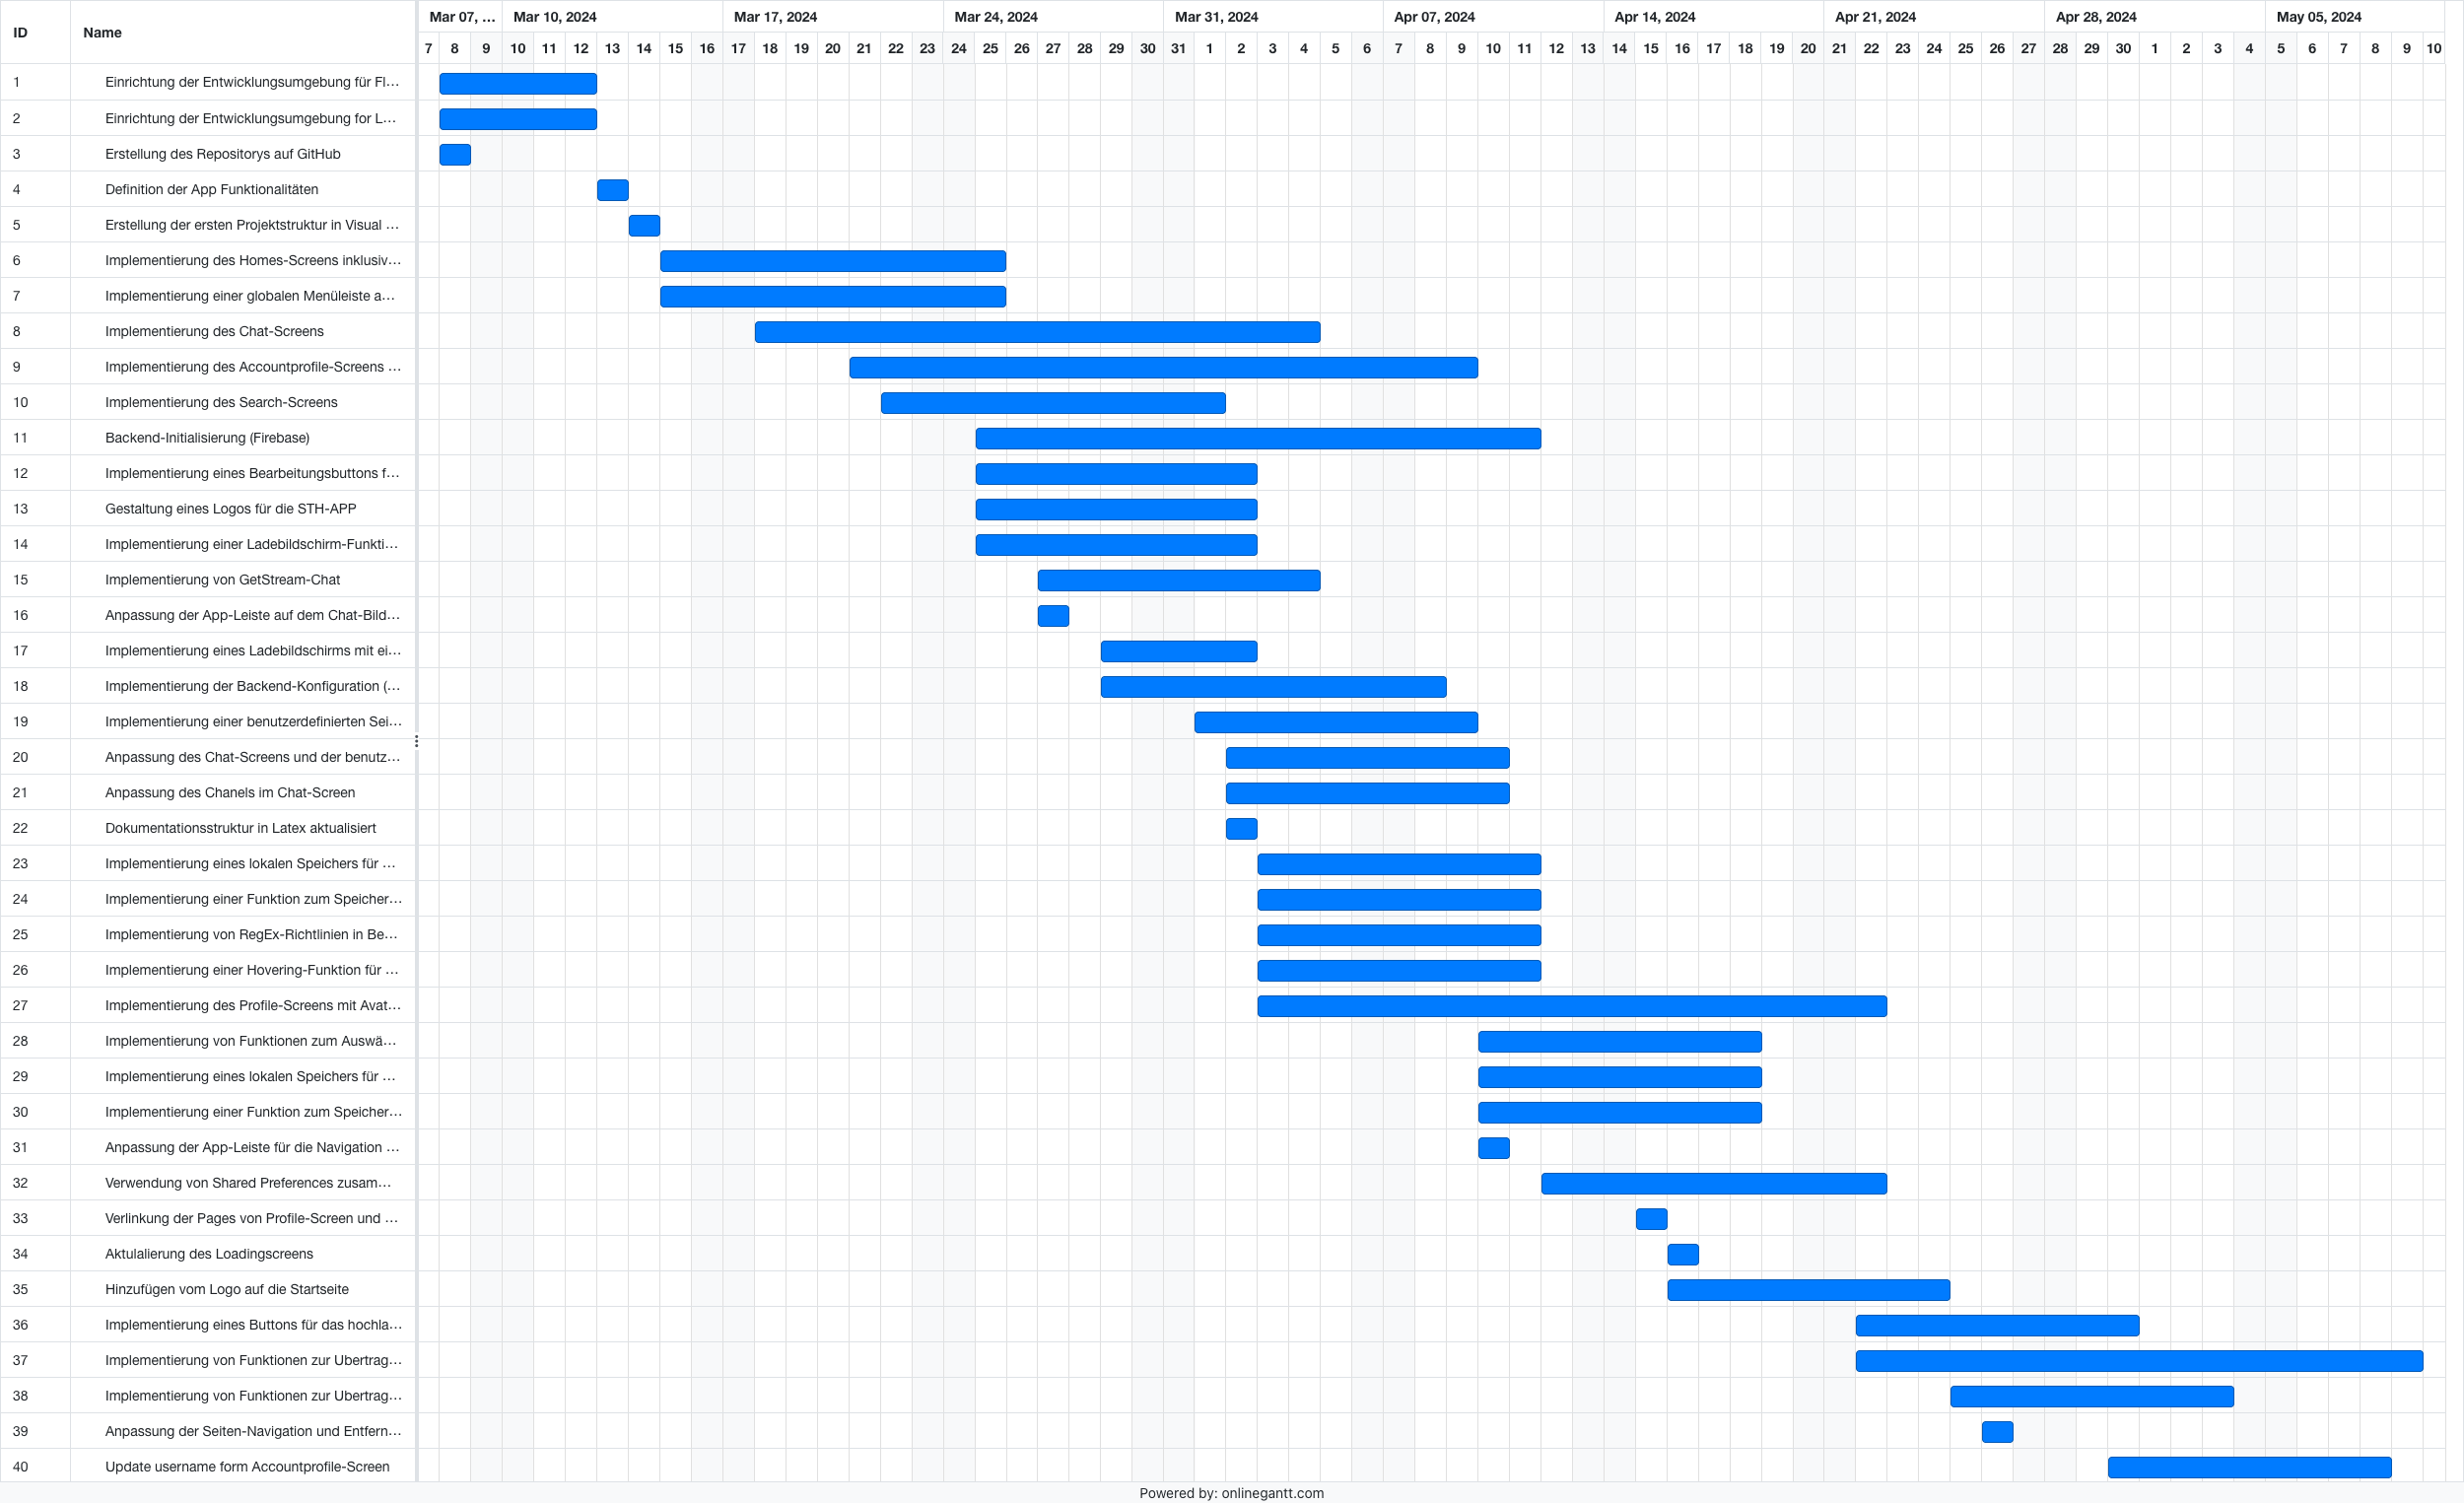
\includegraphics[width=0.9\textwidth]{assets/figures/STH GANTT Diagramm.png}
	\begin{flushleft}
		Quelle: Eigene Darstellung über \url{https://www.onlinegantt.com}
	\end{flushleft}
\end{figure}


